% Source: Lecture23.pdf, pages 1-3. Title on the source: "Analysis of another equation of state (EOS) for gases".
\lecture{23}
\subsection{The Dieterici equation of state}

The van der Waals EOS,
\begin{equation}
  \left[p + a\left(\frac{N}{V}\right)^2\right]\left[V-Nb\right] = N\kB T,
\end{equation}
i.e., with $v\equiv V/N$, the equivalent equation $\left(p + a/v^2\right)(v-b) = \kB T$, was an improvement over the
ideal gas EOS $pV = N\kB T$, i.e.\ $pv = \kB T$, in that it predicted a critical point. The unphysical prediction of
a region with $\partial p/\partial v>0$ and hence compressibility
$\kappa_T = -(1/V)\partial V/\partial p = -(1/v)\partial v/\partial p<0$ could be circumvented via
the Maxwell construction. Recall the solution for $T_c$, $v_c$, and $p_c$ with the vdW EOS:
\begin{equation}
  \kB T_c = \frac{8a}{27b},\qquad v_c = 3b,\qquad p_c = \frac{a}{27b^2},\qquad\text{so}\quad
  Z_c\equiv\frac{p_cv_c}{\kB T_c} = \frac{3}{8} = 0.375,
\end{equation}
with $b = \kB T_c/(8p_c)$ and $a = (27/64)(\kB T_c)^2/p_c$.

The prediction for $Z_c$ is only in fair agreement with experimental values; some of these are (e.g.\ see Table~5.1,
p.~69 in Stanley's book):
\begin{center}
\begin{tabular}{lc@{\hspace{3em}}lc}
  gas & $Z_c$ & gas & $Z_c$\\ \hline
  Xe & 0.288 & H$_2$O & 0.230\\
  Ar & 0.291 & CO$_2$ & 0.275\\
  N$_2$ & 0.291 & CH$_4$ & 0.290\\
  O$_2$ & 0.292 & H$_2$ & 0.304\\
  CO & 0.294 & He & 0.308
\end{tabular}
\end{center}
The first five are all $\simeq 0.29$. So the vdW prediction for $Z_c$ is systematically larger than experimentally
measured values by $\sim 30\%$. This raises the question of whether one can devise a comparably simple EOS that (i)
predicts a smaller value of $Z_c$ in general, and (ii) in particular, predicts a value of $Z_c$ closer to experiment.
(By ``comparably simple'', one means a 2-parameter EOS; obviously one can get a better fit to experimental data with
a multiparameter EOS.) The answer is yes. We next describe one such EOS, called the Dieterici EOS (1899):
\begin{equation}
  p(v-b) = \kB T\exp\left[-\frac{a}{\kB Tv}\right].
\end{equation}
As with vdW, $b$ is an excluded-volume correction and the constant $a$ represents effects of interactions. Clearly,
in the limit $b = 0$ and $a = 0$, this EOS reduces to $pv = \kB T$, as it must. Also, the constants $a$ and $b$ have
the same dimensions as do the corresponding constants $a$ and $b$ in the vdW EOS, namely $[b]\sim$ volume,
$[a]\sim$ energy$\cdot$volume.

Dieterici EOS (DEOS):
\begin{equation}
  p = \frac{\kB T}{v-b}\exp\left[-\frac{a}{\kB Tv}\right].
\end{equation}
Note that expanding the RHS for small $a/(Tv)$ gives
\begin{equation}
  p\simeq\frac{\kB T}{v-b}\left[1-\frac{a}{\kB Tv}\right] = \frac{\kB T}{v-b} - \frac{a}{v(v-b)},
\end{equation}
to be compared with the vdW EOS, $p = \kB T/(v-b) - a/v^2$, so in this expansion, to leading order, the
difference of the DEOS with respect to vdW is the replacement of the denominator in the $a$-term by $v(v-b)$ instead
of $v^2$. Thus, the general shape of the $p$--$v$ curve is qualitatively similar to the vdW $p$--$v$ curve in this
regime.

\begin{diagram}
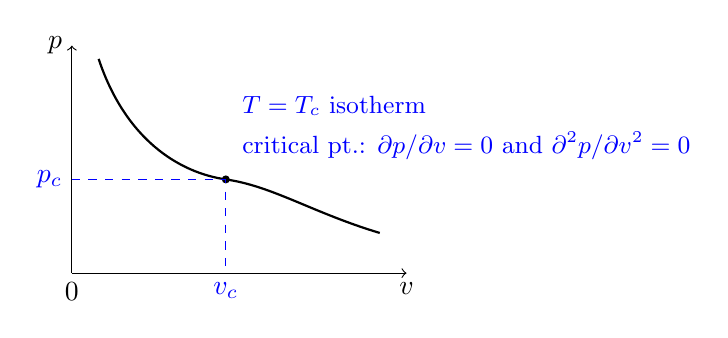
\begin{tikzpicture}[scale=0.85]
  \draw[->] (0,0) -- (5,0) node[below] {$v$}; \draw[->] (0,0) -- (0,3.4) node[left] {$p$};
  \draw[thick] (0.4,3.2) .. controls (0.8,2.0) and (1.6,1.5) .. (2.3,1.4) .. controls (3,1.3) and (3.6,0.9) .. (4.6,0.6);
  \fill (2.3,1.4) circle (0.06);
  \draw[dashed,blue] (0,1.4) -- (2.3,1.4) -- (2.3,0);
  \node[left,blue] at (0,1.4) {$p_c$}; \node[below,blue] at (2.3,0) {$v_c$}; \node[below] at (0,0) {$0$};
  \node[blue,font=\small,anchor=west] at (2.4,2.5) {$T = T_c$ isotherm};
  \node[blue,font=\small,anchor=west,align=left] at (2.4,1.9) {critical pt.: $\partial p/\partial v = 0$ and $\partial^2p/\partial v^2 = 0$};
\end{tikzpicture}
\diagramcaption{The critical isotherm of the Dieterici EOS.}
\end{diagram}

To analyze this EOS, we proceed as before to solve the two equations describing the critical point. It is convenient
to define $\tilde p\equiv\beta p$, $\tilde a\equiv\beta a$, so
\begin{equation}
  \text{DEOS:}\quad \beta p = \frac{e^{-\beta a/v}}{v-b},\qquad \tilde p = \frac{e^{-\tilde a/v}}{v-b}.
\end{equation}
Since $\beta$ = const.\ on an isotherm, $\partial p/\partial v = 0\Leftrightarrow\partial \tilde p/\partial v = 0$:
\begin{equation}
  \pder{\tilde p}{v} = \frac{\tilde a}{v^2}\frac{e^{-\tilde a/v}}{v-b} - \frac{e^{-\tilde a/v}}{(v-b)^2}
  = \frac{e^{-\tilde a/v}}{v-b}\left[\frac{\tilde a}{v^2} - \frac{1}{v-b}\right] = 0
  \ \Rightarrow\ \frac{1}{v-b} = \frac{\tilde a}{v^2}.
\end{equation}
Similarly, $\partial^2p/\partial v^2 = 0\Leftrightarrow\partial^2\tilde p/\partial v^2 = 0$:
\begin{align}
  0 = \frac{\partial^2\tilde p}{\partial v^2}
   &= -\frac{2\tilde a}{v^3}\frac{e^{-\tilde a/v}}{v-b} + \frac{\tilde a}{v^2}\cdot\frac{\tilde a}{v^2}\frac{e^{-\tilde a/v}}{v-b}
      \underbrace{- \frac{\tilde a}{v^2}\frac{e^{-\tilde a/v}}{(v-b)^2} - \frac{\tilde a}{v^2}\frac{e^{-\tilde a/v}}{(v-b)^2}}_{-(2\tilde a/v^2)e^{-\tilde a/v}/(v-b)^2}
      + \frac{2e^{-\tilde a/v}}{(v-b)^3}\nonumber\\
   &= \frac{e^{-\tilde a/v}}{v^3(v-b)}\left[-2\tilde a + \frac{\tilde a^2}{v} - \frac{2\tilde av}{v-b} + \frac{2v^3}{(v-b)^2}\right].
\end{align}
In $\partial^2\tilde p/\partial v^2$, we replace $1/(v-b)$ by $\tilde a/v^2$ using the first
condition:
\begin{equation}
  = \frac{1}{v^3}\frac{\tilde a}{v^2}e^{-\tilde a/v}\left[-2\tilde a + \frac{\tilde a^2}{v}
    \underbrace{-\,2\tilde av\left(\frac{\tilde a}{v^2}\right)}_{-2\tilde a^2/v}
    \underbrace{+\,2v^3\left(\frac{\tilde a}{v^2}\right)^2}_{+2\tilde a^2/v}\right],
\end{equation}
where the last two terms cancel, so
\begin{equation}
  0 = \frac{\partial^2\tilde p}{\partial v^2} = \frac{\tilde a^2}{v^5}e^{-\tilde a/v}\left(-2+\frac{\tilde a}{v}\right)
  \ \Rightarrow\ \tilde a = 2v .
\end{equation}
Next, substitute this into the $\partial \tilde p/\partial v = 0$ equation: $1/(v-b) = \tilde a/v^2 = 2/v$
$\Rightarrow v-b = v/2$, $v/2 - b = 0\Rightarrow$
\begin{equation}
  \boxed{v = v_c = 2b},\qquad\text{so}\quad \tilde a = \beta a = \frac{v^2}{v-b} = \frac{(2b)^2}{b} = 4b,
\end{equation}
\begin{equation}
  \Rightarrow\quad\boxed{\beta = \beta_c = \frac{4b}{a},\quad \kB T_c = \frac{1}{\beta_c} = \frac{a}{4b}}.
\end{equation}
Then
\begin{equation}
  p = p_c = \frac{\kB T_c}{v_c-b}e^{-\beta_ca/v_c} = \frac{\left(a/(4b)\right)}{b}\underbrace{\exp\left[-\frac{\left(4b/a\right)a}{2b}\right]}_{e^{-2}},
  \qquad\text{so}\quad\boxed{p_c = \frac{a}{4b^2}e^{-2}}.
\end{equation}

\paragraph{Summary for the Dieterici EOS.}

\begin{gather}
  p = \frac{\kB T}{v-b}\exp\left[\frac{-a}{\kB Tv}\right],\quad\text{i.e.}\quad p = \frac{\beta^{-1}}{v-b}e^{-\beta a/v};\nonumber\\
  v_c = 2b,\quad \kB T_c = \beta_c^{-1} = \frac{a}{4b},\quad p_c = \frac{a}{4b^2}e^{-2}.
\end{gather}
Then
\begin{equation}
  Z_c\equiv\frac{p_cv_c}{\kB T_c} = \frac{\left(a/(4b^2e^2)\right)(2b)}{\left(a/(4b)\right)}
  \ \Rightarrow\ \boxed{Z_c = \frac{2}{e^2} = 0.27067},
\end{equation}
where $e = 2.71828\ldots$. Determining $a$ and $b$ from $T_c$ and $p_c$:
\begin{equation}
  b = \frac{v_c}{2} = \frac{1}{2}\left(\frac{\kB T_cZ_c}{p_c}\right) = \frac{1}{e^2}\left(\frac{\kB T_c}{p_c}\right);\qquad
  a = (4b)(\kB T_c) = \left(\frac{2}{e}\right)^2\frac{(\kB T_c)^2}{p_c}.
\end{equation}
So the Dieterici EOS predicts a smaller value of $Z_c$ than the van der Waals EOS, closer to experimental values, about
7\% below the $Z_c\simeq 0.29$ values for Xe, Ar, N$_2$, O$_2$, and close to $Z_c = 0.275$ for CO$_2$, for example.

\subsubsection*{Comparison of the van der Waals and Dieterici equations of state}

\begin{equation*}
  \text{vdW EOS:}\quad p = \frac{\kB T}{v-b} - \frac{a}{v^2}\qquad\Big|\qquad
  \text{DEOS:}\quad p = \frac{\kB T}{v-b}\exp\left[-\frac{a}{\kB Tv}\right]
\end{equation*}
Critical values:
\begin{center}
\small\renewcommand{\arraystretch}{1.6}\setlength{\tabcolsep}{4pt}
\begin{tabular}{l|l|l}
  quantity & van der Waals & Dieterici\\ \hline
  $v_c$ & $3b$ & $2b$\\
  $p_c$ & $a/(27b^2) = 0.0370\,a/b^2$ & $a/(4e^2b^2) = 0.0338\,a/b^2$\\
  $\kB T_c$ & $8a/(27b) = 0.296\,a/b$ & $a/(4b) = 0.25\,a/b$\\
  $Z_c = p_cv_c/(\kB T_c)$ & $3/8 = 0.375$ & $2/e^2 = 0.271$\\
  $a$ & $(27/64)(\kB T_c)^2/p_c = 0.422(\kB T_c)^2/p_c$ & $(4/e^2)(\kB T_c)^2/p_c = 0.541(\kB T_c)^2/p_c$\\
  $b$ & $\kB T_c/(8p_c) = 0.125\,\kB T_c/p_c$ & $\kB T_c/(e^2p_c) = 0.135\,\kB T_c/p_c$
\end{tabular}
\end{center}
A modern discussion of the Dieterici EOS is in R.~Sadus, J.\ Chem.\ Phys.\ \textbf{115}, 1460 (2001).
